\documentclass[12pt]{aghdpl}

\usepackage[english,polish]{babel}

% Użyj polskiego łamania wyrazów (zamiast domyślnego angielskiego).
\usepackage{polski}

\usepackage[utf8]{inputenc}

% dodatkowe pakiety

\usepackage{mathtools}
\usepackage{amsfonts}
\usepackage{amsmath}
\usepackage{amsthm}

% --- < bibliografia > ---

\usepackage[
style=numeric,
sorting=none,
%
% Zastosuj styl wpisu bibliograficznego właściwy językowi publikacji.
language=autobib,
autolang=other,
% Zapisuj datę dostępu do strony WWW w formacie RRRR-MM-DD.
urldate=iso8601,
% Nie dodawaj numerów stron, na których występuje cytowanie.
backref=false,
% Podawaj ISBN.
isbn=true,
% Nie podawaj URL-i, o ile nie jest to konieczne.
url=false,
%
% Ustawienia związane z polskimi normami dla bibliografii.
maxbibnames=3,
% Jeżeli używamy BibTeXa:
backend=bibtex
]{biblatex}

\usepackage{csquotes}
% Ponieważ `csquotes` nie posiada polskiego stylu, można skorzystać z mocno zbliżonego stylu chorwackiego.
\DeclareQuoteAlias{croatian}{polish}

\addbibresource{bibliografia.bib}

% Nie wyświetlaj wybranych pól.
%\AtEveryBibitem{\clearfield{note}}


% ------------------------
% --- < listingi > ---

% Użyj czcionki kroju Courier.
\usepackage{courier}

\usepackage{listings}
\lstloadlanguages{TeX}

\lstset{
	literate={ą}{{\k{a}}}1
           {ć}{{\'c}}1
           {ę}{{\k{e}}}1
           {ó}{{\'o}}1
           {ń}{{\'n}}1
           {ł}{{\l{}}}1
           {ś}{{\'s}}1
           {ź}{{\'z}}1
           {ż}{{\.z}}1
           {Ą}{{\k{A}}}1
           {Ć}{{\'C}}1
           {Ę}{{\k{E}}}1
           {Ó}{{\'O}}1
           {Ń}{{\'N}}1
           {Ł}{{\L{}}}1
           {Ś}{{\'S}}1
           {Ź}{{\'Z}}1
           {Ż}{{\.Z}}1,
	basicstyle=\footnotesize\ttfamily,
}

% ------------------------

\AtBeginDocument{
	\renewcommand{\tablename}{Tabela}
	\renewcommand{\figurename}{Rys.}
}

% ------------------------
% --- < tabele > ---

\usepackage{array}
\usepackage{tabularx}
\usepackage{multirow}
\usepackage{booktabs}
\usepackage{makecell}
\usepackage[flushleft]{threeparttable}

% defines the X column to use m (\parbox[c]) instead of p (`parbox[t]`)
\newcolumntype{C}[1]{>{\hsize=#1\hsize\centering\arraybackslash}X}


%---------------------------------------------------------------------------

\author{Amadeusz Hercog}
\shortauthor{A. Hercog}

%\titlePL{Przygotowanie bardzo długiej i pasjonującej pracy dyplomowej w~systemie~\LaTeX}
%\titleEN{Preparation of a very long and fascinating bachelor or master thesis in \LaTeX}

\titlePL{Wykorzystanie algorytmu sztucznej inteligencji do rozwiązania problemu optymalnego wyboru ścieżki lub wyjścia ewakuacyjnego}
\titleEN{}


\shorttitlePL{Rozwiązanie problemu optymalnego wyboru ścieżki lub wyjścia ewakuacyjnego} % skrócona wersja tytułu jeśli jest bardzo długi
\shorttitleEN{}

\thesistype{Praca dyplomowa inżynierska}
%\thesistype{Master of Science Thesis}

\supervisor{mgr. inż. Robert Lubaś}
%\supervisor{Marcin Szpyrka PhD, DSc}

\degreeprogramme{Informatyka stosowana}
%\degreeprogramme{Computer Science}

\department{Wydział Informatyki Stosowanej}
%\department{Department of Applied Computer Science}

\faculty{Wydział Fizyki i Informatyki}
%\faculty{Faculty of Electrical Engineering, Automatics, Computer Science and Biomedical Engineering}

\acknowledgements{Serdecznie dziękuję \dots tu ciąg dalszych podziękowań np. dla promotora, żony, sąsiada itp.}

\setlength{\cftsecnumwidth}{10mm}

%---------------------------------------------------------------------------
\setcounter{secnumdepth}{4}
\brokenpenalty=10000\relax

% arial
\renewcommand{\rmdefault}{phv}
\renewcommand{\sfdefault}{phv}

% wyłączenie łamania słów i justowanie
\usepackage[none]{hyphenat}
\sloppy

% wcięcie na pierwszych liniach rozdziałów
\usepackage{indentfirst}

% klikalne linki
\usepackage[colorlinks, linkcolor=blue]{hyperref}

% dane dokumentu
\title{Wykorzystanie algorytmu sztucznej inteligencji do rozwiązania problemu optymalnego wyboru ścieżki lub wyjścia ewakuacyjnego}
\author{Amadeusz Hercog}
\date{21 listopada 2018}

% ładnie wystylizowana tabela
\usepackage[table, svgnames]{xcolor} \usepackage{array}
\usepackage{etoolbox}

\definecolor{table_header_color}{HTML}{B0BEC5}
\definecolor{even_row_color}{HTML}{EEEEEE}

\newenvironment{tightcenter}{
  \setlength\topsep{0pt}
  \setlength\parskip{0pt}
  \begin{center}
}{
  \end{center}
}

\newenvironment{mytabular}{\rowcolors{1}{\ifnumless{\rownum}{2}{table_header_color}{even_row_color}}{}\begin{tightcenter}\tabular}{\endtabular\end{tightcenter}}

%centrowanie nagłówków
\captionsetup{justification=centering}

\begin{document}
	\titlepages
	
	\chapter{Wstęp}
	\textit{W tym rozdziale zostanie opisane podłoże historyczne, cel i jego założenia projektu. Zaprezentowane zostanie proponowane rozwiązanie postawionego problemu oraz technologie do tego użyte.}
	
		\section{Cel projektu}	
		W wielu miastach miastach, gdzie istnieją duże skupiska ludzi prędzej czy później pojawia się problem alokacji przestrzeni na zabudowę. W tym celu nowoczesne budynki uzytku publicznego są projektowane pod kątem wykorzystania jak największej przestrzeni dla celów użytkowych, ale i z drugiej strony - dla zapewnienia jak największego bezpieczeństwa ludziom w nich przebywających. Jednym z czynników określających wchodzącym w skład szeroko pojętego bezpieczeństwa, jest zapewnienie ludziom ścieżek ewakuacyjnych w razie pożaru lub innych wypadków. Z tego powodu celu postawiłem następujący problem - rozwiązanie problemu optymalizacji wyboru ścieżki lub wyjścia ewakuacyjnego ludzi w budynku. Co więcej, w związku z moim wcześniejszym doświadczeniem z tematem uczenia maszynowego, postanowiłem rozwiązać ten problem za pomocą technik machine learning.
		
		\section{Użyte technologie oraz programy}
		Wszystkie obliczenia oraz rysowanie wykresów zostało zrealizowane w języku programowania \textbf{Python} w wersji 3.6 przy użyciu bibliotek:
		\begin{itemize}
			\item \textbf{NumPy} - służąca do obliczeń numerycznych,
			\item \textbf{Pandas} - słuzaca łatwiejszemu zarządzaniu duzą ilością danych,
			\item \textbf{Matplotlib} - służąca do rysowania wykresów,
			\item \textbf{Tensorflow} - używana do głębokiego uczenia maszynowego.
		\end{itemize}
		
		Aby mieć możliwość symulacji ruchu pieszych w budynku, użyłem symulatora \textbf{PSP} \textit{(Pederastian Simulation Project)} autorstwa Roberta Lubaś oraz Wojciecha Myśliwiec - opisany szerzej w rozdziale~\ref{sekcja_psp}.
		
		\section{Proponowane rozwiązanie}
		Rozwiązanie proponowane przeze mnie zostało podzielone na kilka kroków:
		\begin{enumerate}
		\item\label{proponowane_rozwiazanie_generacja_danych} Wygenerowanie \textit{n} zestawów parametrów wejściowych do symulatora \textit{PSP} w celu pozyskania jego danych wyjściowych.
		\item Stworzenie modelu uczenia maszynowego na podstawie wygenerowanych zestawów danych wejściowych oraz wyjściowych symulatora i nauczenie go na danych z punktu~\ref{proponowane_rozwiazanie_generacja_danych}. Daje to możliwość generowania nowych danych wyjściowych bez używania symulatora.
		\item Optymalizacja zestawu danych wyjściowych modelu na podstawie jego danych wejściowych używając metod optymalizacji.
		\end{enumerate}
	
	\newpage
	\chapter{PSP - Pederastian Simulator Project}\label{sekcja_psp}
	\textit{W tym rozdziale opisany zostanie symutalor ruchu pieszych użyty w projekcie i jego sposób użycia wraz z potrzebnymi dodatkowymi plikami. Opisane zostaną użyte w projekcie parametry wejściowe do symulatora oraz metryki stworzone na podstawie jego danych wyjściowych.}
	
		\section{Opis}
		Symulator \textit{Pederastian Simulator Project} jest programem napisanym w języku C++ autorstwa Roberta Lubaś oraz Wojciecha Myśliwiec. Służy on do modelowania ruchu agentów (ludzi) podczas ewakuacji w danej przestrzeni. Symulowana przestrzeń jest dwuwymiarowa, z możliwością dodania wielu poziomów odpowiadających kolejnym piętrom budynku. Główne okno programu jest widoczne na rysunku~\ref{fig: glowne_okno_symulatora}.
	
		\begin{figure}[h]
	 		\begin{tightcenter}
	 			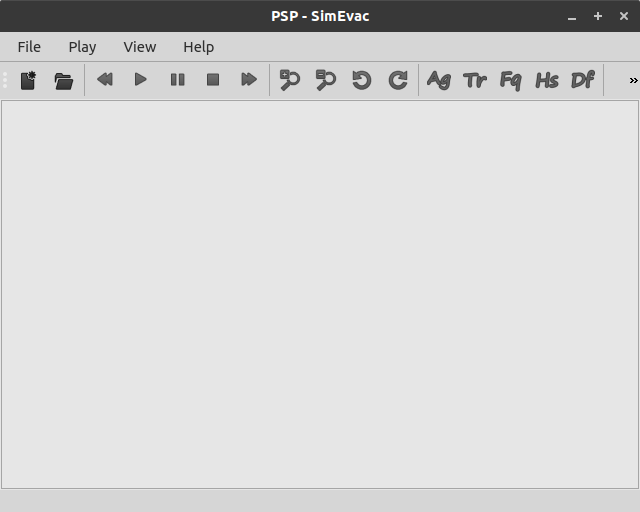
\includegraphics[width = 0.75\linewidth]{rysunki/symulator.png}
	 		\end{tightcenter}
	 		
			\caption{Główne okno symulatora.}
			\label{fig: glowne_okno_symulatora}
		\end{figure}
	
		\section{Sposób użycia}
		Do przeprowadzenia symulacji potrzebne są następujące rzeczy:
		\begin{itemize}
		\item plik \textit{.xml} zawierający parametry wejściowe symulacji,
		\item pliki \textit{.jpg} i \textit{.bmp} zwierające przestrzeń użytą do symulacji.
		\end{itemize}
	
		W oknie głównym programu należy wybrać opcje otwarcia pliku \textit{.xml} po czym od razu zaczyna się symulacja w czasie rzeczywistym. Po symulacji, we wskazanym w pliku z parametrami folderze zostaną wygenerowane pliki \textit{.csv} z danymi wyjściowymi symulacji.
		
		\section{Dane wejściowe i wyjściowe}
		Dane, na których miałem możliwość przeprowadzenia badań znajdowały się w:
		\begin{itemize}
		\item dane wejściowe - plik \textit{.xml},
		\item dane wyjściowe - pliki \textit{.csv}.
		\end{itemize}
		
		Danymi wejściowymi, które wybrałem - na podstawie łatwości modyfikacji - do dalszej analizy były:\label{dane_do_dalszej_analizy}
		
		\begin{itemize}
		\item \textbf{Panic spread factor} - współczynnik, który decyduje jak duzy wpływ ma \textbf{tryb paniki} (tryb, w którym agenci zwracają mniejszą uwagę na otoczenie oraz charakteryzują się bardziej chaotycznym ruchem) na agentów.
		\item \textbf{Panic cancel zone} - współczynnik określający odległość od wyjść, w obrębie jakiej agenci mają szansę na deaktywację trybu paniki.
		\item \textbf{Cancel panic chance}- podczas testów na anulowanie trybu paniki określa procent szans na powodzenie.
		\item \textbf{Choosing evacuation path mode} - tryb wyboru drogi ewakuacyjnej przez agentów. Dostępne są 4 tryby:
			\begin{itemize}
			\item odległości,
			\item gęstości przy wyjściu,
			\item odległości oraz gęstości przy wyjściu,
			\item odległości, gęstości przy wyjściu oraz popularności wyboru wyjścia.
			\end{itemize}
		\item \textbf{Number of pederastians} - liczba agentów biorąca udział w symulacji.
		\item \textbf{Chaos level} - szansa na aktywację trybu paniki u agentów.
		\item \textbf{Density factor} - określa wpływ współczynnika gęstości wokół agenta na funkcję kary.
		\item \textbf{Frequency factor} - określa wpływ częstości wyboru danego pola na funkcję kary.
		\item \textbf{Panic factor} - potęguje część współczynników biorących udział w obliczaniu funkcji kary. 
		\item \textbf{Distance factor} - wpływa na wybór agentów ruchu po skosie lub na wprost.
		\item \textbf{Randomness factor} - czynnik losowości dla wartości kary.
		\item \textbf{Pre-movement time mean value} oraz \textbf{Pre-movement time standard deviation} - średnia i odchylenie czasu \textit{Pre-movement}, który ma wpływ na częstotliwość wykonywania testu na zmianę obranego wyjścia przez agentów.
		\item \textbf{Speed distribution mean value} oraz \textbf{Speed distribution standard deviation} - średnia i odchylenie prędkości agentów.
		\end{itemize}
		
		Dane wyjściowe wybrane wybrane do analizy przeze mnie były następujące:
		
		\begin{itemize}
		\item czas ewakuacji osatatniego agenta (odpowiadający czasowi ewakuacji wszystkich agentów),
		\item błąd średniokwadratowy średnich prędkości wszystkich agentów w stosunku do średniej prędkości najszybszego agenta.
		\end{itemize}
		
		Dodatkowe parametry wejściowe, które były mi potrzebne (lecz nie wpływały na sam proces badawczy) to:
		\begin{itemize}
		\item \textbf{Repeat number} - ilość powtórzeń symulacji wykonanej na pojedynczym pliku \textit{.xml}.
		\item \textbf{Sim directory} - określa ścieżkę do folderu zawierającego pliki symulowanej przestrzeni.
		\item \textbf{Sim stat directory} - określa ścieżkę do folderu, do którego zostaną zapisane dane wyjściowe symulacji (pliki \textit{.csv}).
		\end{itemize}
		
	\newpage
	\chapter{Budowa projektu}
	\textit{W tym rozdziale opisany będzie proces zbierania danych za pomocą symulatora PSP, tworzenie modelu uczenia maszynowego oraz optymalizacji jego wartości wyjściowych.}
	
		\section{Zebranie danych}
		W celu zebrania danych, które miałyby trafić później do modelu uczenia maszynowego, stworzyłem skrypt pythonowy, który wygenerował 200 różnych zestawów parametrów wejściowych do symulatora. Rodzaje danych, które wygenerowałem znajdują się w rozdziale~\ref{dane_do_dalszej_analizy}. Dla każdego zestawu danych ustawiłem parametrowi \textit{Repeat number} wartość 10, dzięki czemu dla każdego zestawu danych wejściowych generowane było 10 zestawów danych wyjściowych. Było to niezwykle cenne z 2 powodów:
		\begin{itemize}
		\item Do symulatora trzeba było ręcznie ładować plik \textit{.xml}, a dzięki temu z jedngo pliku otrzymywałem od razu 10 zestawów plików wyjściowych.
		\item Ruchy agentów, nawet z takim samym zestawem parametrów, rożnią się między symulacjami, a dzięki powtórzeniom łatwiej było wyeliminować te różnice.
		\end{itemize}
		
		Dla części symulacji, symulator niespodziewanie wyłączył się podczas pracy, przez co niektórym zestawom danych wejściwych odpowiada mniej niż 10 zestawów danych wyjściowych. Ostatecznie z 200 zestawów parametrów wejściowych uzyskałem 1888 zestawów parametrów wyjsciowych. Oznacza to, że 5,6\% z symulacji, które miały zostać przeprowadzone nie udały się.	
		
		W pierwszym podejściu, aby móc przetestować model w prostych warunkach, wybrałem z kazdego zestawu danych: wszystkie dane wejściowe, jedną daną wyjściową. Daną wyjściową, którą wybrałem był czas ewakuacji ostatniego agenta. Każdy zestaw danych zawierał więc \textbf{15} parametrów wejściowych oraz \textbf{1} parametr wyjściowy. Z tak przygotowanymi danymi miałem możliwość wybrania pierwszego modelu.
		
		\section{Opis modelu Perceptron}		
		Na poczatek, wybrałem prosty model uczenia maszynowego - regresję liniową. Stworzyłem go wykorzystując \textbf{Perceptron}. Jest to prosta sieć neuronowa, która posiada zestaw neuronów wejściowych, kazdy odpowiadający pojedynczej danej wejsciowej. Składa się on także z jednego lub wielu niezależnych neuronów wyjściowych. Każdy z nich jest połączony ze wszystkimi neuronami wejściowymi za pomocą krawędzi posiadających wagi - definiują one jak duży wpływ na wyjście ma każda dana wejściowa. Jeśli wyrazimy:
		\begin{itemize}
		\item wejście jako wektor \textit{X},
		\item wyjście pojedyczego Perceptronu jako \textit{a},
		\item neuron jako wektor wag \textit{N},
		\item funkcję aktywacji jako $\sigma$ - jest to funkcja wprowadzająca nieliniowość danych, najpopularniejsze z nich to \textit{Sigmoid}, \textit{ReLU (Rectified linear unit)} czy też \textit{Softmax}
		\end{itemize}
		to zachodzi równanie:
		
		\begin{equation}
		Y=\sigma(NX)
		\end{equation}
	
		Budowa Perceptronu z jednym neuronem wyjściowym jest widoczna na rysunku \ref{fig: budowa_perceptronu}\footnote{\url{https://pythonmachinelearning.pro/perceptrons-the-first-neural-networks/}}.

		\begin{figure}[h]
	 		\begin{tightcenter}
	 			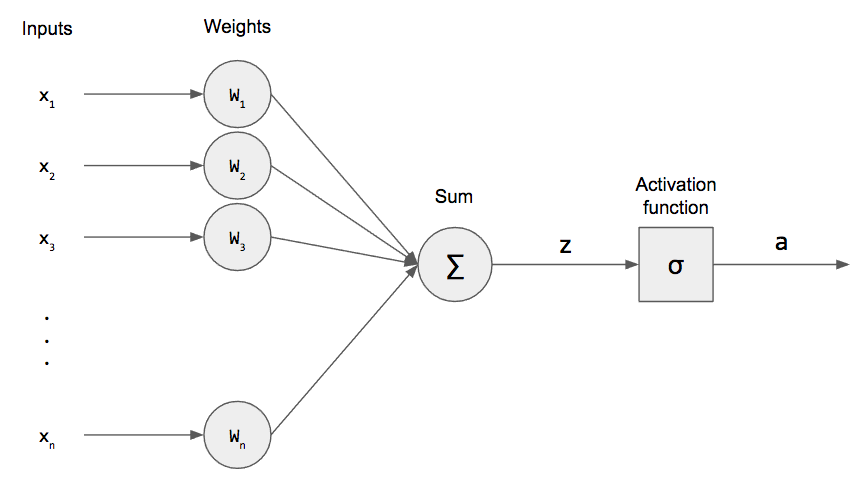
\includegraphics[width = 0.75\linewidth]{rysunki/perceptron.png}
			\end{tightcenter}	 			
	 			
 			\caption{Budowa Perceptronu z jednym neuronem wyjściowym.}
			\label{fig: budowa_perceptronu}
		\end{figure}

		Podczas procesu uczenia \textit{Perceptronu} ważne jest aby określić \textbf{loss function} - metrykę którą chcemy optymalizować. Dla problemów regresji najczęściej uzywaną funkcją kosztu jest \textbf{MSE} (Mean Squared Error). Kolejnym parametrem sieci \textit{Perceptron} jest parametr \textbf{learning rate}, który określa jak bardzo będzie się zmieniać macierz/wektor wag na podstawie gradientu podczas każdej iteracji uczącej. Zbyt duży współczynnik \textit{learning rate} może spowodować, że zamiast optymalizować funkcję kosztu będzie wręcz przeciwnie - będzie ona osiągała coraz większe wartości. Gdy jest on zbyt mały, jest on mniej niebezpieczny gdyż nie doprowadzi on do wzrostu wartości funkcji kosztu; problemem jest jednak wolniejszy proces uczący sieci co wymaga więcej epok uczących. Nie ma jednak uniwersalnej metody regulującej sposób dobierania \textit{learning rate} - trzeba to robić eksperymentalnie.
		
		\section{Pierwszy model - tworzenie i analiza} \label{pierwszy_model_tworzenie_i_analiza}
		Dla powyższych zastosowań stworzyłem więc \textit{Perceptron} posiadający pojdeyncze wyjście oraz nie posiadający funkcji aktywacji - jako że model miał służyć do regresji a nie klasyfikacji. Zestawy danych podzieliłem w stosunku 80\% : 20\% na \textbf{dane treningowe} i \textbf{dane testowe}, pozwala to na trenowanie sieci na danych treningowych oraz sprawdzanie jej efektowności na tanych testowych co daje możliwość walidacji tego, jak dobrze sieć radzi sobie z danymi, z którymi nie miała styczności.
		
		Podsumowując, parametry pierwszego modelu były więc następujące:
		\begin{itemize}
		\item pojedyncza warstwa składająca się z jednego neuronu,
		\item \textbf{funkcja aktywacji} - brak,
		\item \textbf{learning rate} - 0.1,
		\item \textbf{metryka do optymalizacji} - MSE,
		\item \textbf{liczba epok uczacych} - 300,
		\item podział na \textbf{dane treningowe} i \textbf{dane testowe} - 80\% : 20\%.
		\end{itemize}
				
		Proces uczący został wykonany 10 razy od nowa na nienauczonym modelu, za kazdym razem wykonując permutację danych. Średnie \textit{MSE} danych wyglądają następująco:
		\begin{itemize}
		\item \textbf{średnia i odchylenia MSE danych treningowych} - ($\pm$),
		\item \textbf{średnia i odchylenia MSE danych testowych} - ($\pm$).
		\end{itemize}
		Najlepszy przypadek (biorąc pod uwagę \textit{MSE} danych testowych jest następujący:
		\begin{itemize}
		\item \textbf{MSE danych treningowych} - ,
		\item \textbf{MSE danych testowych} - .
		\end{itemize}
		Zależność \textit{MSE} danych od iteracji uczacej tego przypadku jest widoczna na wykresie \ref{fig: pierwszy_model_wykres_uczenia}. Analizując go, doszedłem do następujących wniosków:
		\begin{itemize}
		\item \textit{MSE} danych treningowych jak i testowych jest na wysokim poziomie co oznacza, że model ma \textbf{wysoki bias}. Oznacza to, że użyty model jest zbyt prosty i nie ważne jak dużo danych zostanie do niego podanych i jak długo będzie się on uczył - \textit{MSE} danych nie obniży się poniżej pewnego poziomu.
		\item Podczas uczenia \textit{MSE} danych jest bardzo niestabilny, co oznacza niestabilność danych lub modelu.
		\item \textit{MSE} danych testowych jest przez większośc iteracji mniejsze niż treningowych co oznacza, że dla danych których sieć nie widziała, przewiduje ona wartości bliższe prawdzie niż na danych na których się uczyła. Jest to niecodzienne zachowanie co również dowodzi niestabilności modelu lub danych.
		\end{itemize}
		
		\begin{figure}[h]
	 		\begin{tightcenter}
	 			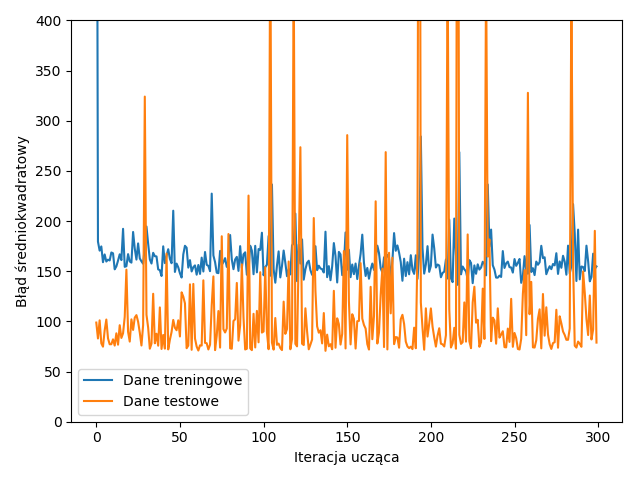
\includegraphics[width = 0.75\linewidth]{rysunki/pierwszy_model_wykres_uczenia.png}
	 		\end{tightcenter}
	 		
 			\caption{Zależność \textit{MSE} danych od iteracji uczącej dla najlepszego przypadku w pierwszym modelu.}
			\label{fig: pierwszy_model_wykres_uczenia}
		\end{figure}
		
		Aby mieć szerszy pogląd na to jaki wpływ ma ilość danych na których się uczy sieć na \textit{MSE} tych danych postanowiłem	uruchomić proces uczacy kolejne 20 razy dla pojedynczej permutacji danych wejściowych, lecz przy zwiększającej się ilości danych treningowych. Wynik tego badania jest widoczny na wykresie \ref{fig: pierwszy_model_learning_curves}. Informacją jaką można z niego wyciągnąć jest ilość danych potrzebna do tego aby osiągnąć dany pułap \textit{MSE} danych. Widać że podczas gdy przy danych treningowych, większa ich ilość spowodowała spadek ich \textit{MSE} to przy danych testowych nie spowodowało to większej różnicy.
		
		\begin{figure}[h]
	 		\begin{tightcenter}
	 			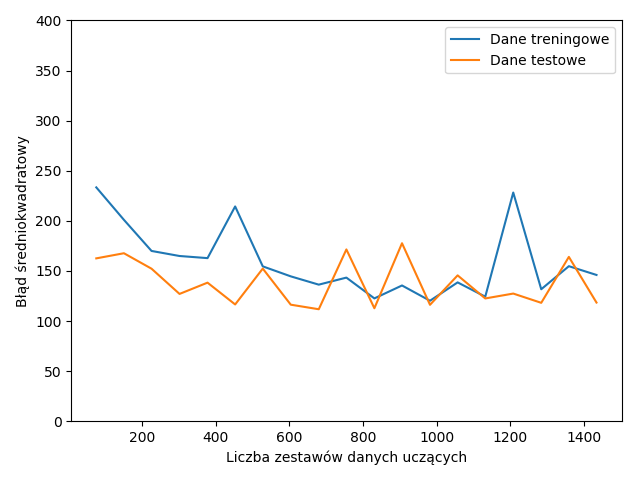
\includegraphics[width = 0.75\linewidth]{rysunki/pierwszy_model_learning_curves.png}
	 		\end{tightcenter}
	 		
 			\caption{Zależność \textit{MSE} danych od ich ilości w pierwszym modelu.}
			\label{fig: pierwszy_model_learning_curves}
		\end{figure}
		
		Podsumowując, obecny model ma wysoki bias - jest zbyt prosty dla danych, przez co większa ich ilość oraz dłuższy proces uczący nie dają żadnych efektów. Na wykresach widać niestabilność modelu lub danych, co powoduje bardzo duże szumy na wykresach \textit{MSE}. Co więcej - niepokojący jest fakt, że \textit{MSE} danych testowych był przeważnie inższy niż \textit{MSE} danych treningowych.
		
		\section{Normalizacja danych}
		Mając na uwadze problemy stworzonego modelu, w pierwszej kolejności postanowiłem przejrzeć dane wejściowe do modelu. Ze wszystkich zestawów danych obliczyłem więc średnią każdego z parametrów wejściowych do sieci neuronowej. Wyniki są widoczne w tabeli \ref{srednie_wartosci_i_odchylenia_parametrow_wejsciowych_modelu}. Widać w niej, że niektóre parametry mają wartości 2 rzędy wielkości większe niż inne. Takie różnice pomiędzy różnymi parametrami wejściowymi powodują faworyzowanie przez sieć jednych parametrów ponad drugie. Postanowiłem więc zastosować normalizację danych według wzoru:
		
		\begin{equation}
		X_{new} = \frac{X_{old} - \mu}{\sigma}
		\end{equation}		 
		
		Gdzie:
		\begin{itemize}
		\item $\mu$ - wektor średniej parametrów,
		\item $\sigma$ - wektor odchylenia parametrów.
		\end{itemize}
		
		\begin{table}[t]
			\caption{Średnie wartości i odchylenia parametrów wejściowych do modelu.}
			\begin{mytabular}{r c c}
					\multicolumn{1}{c}{Nazwa parametru} & Średnia wartość \\
					Panic spread factor & 1.74 \\
					Panic cancel zone & 0.53 \\
					Cancel panic chance& 51.59 \\
					Choosing evacuation path mode & 2.53 \\
					Number of pederastian& 271.8 \\
					Chaos level & 53.9 \\
					Density factor & 5.26 \\
					Frequency factor & 5.33 \\
					Panic factor & 1.45 \\
					Distance factor & 2.51 \\
					Randomness factor & 0.49 \\
					Pre-movement time mean value & 5.44 \\
					Pre-movement time standard deviation & 0.51 \\
					Speed distribution mean value & 5.62 \\
					Speed distribution standard deviation & 0.54
			\end{mytabular}
			\label{srednie_wartosci_i_odchylenia_parametrow_wejsciowych_modelu}
		\end{table}
		
		Posiadając tak przygotowane dane wykonałem - tak jak w punkcie \ref{pierwszy_model_tworzenie_i_analiza} - 10 cykli nauczania z różnymi permutacjami danych oraz 20 cykli z jedną permutacją, lecz zmieniającym się rozmiarem zestawu danych treningowych. Średnie \textit{MSE} danych są następujące:
		\begin{itemize}
		\item \textbf{średnia i odchylenia MSE danych treningowych} - 154,79 ($\pm$),
		\item \textbf{średnia i odchylenia MSE danych testowych} - 78,88 ($\pm$).
		\end{itemize}
		Najlepszy wynik spośród cyklów z różnymi permutacjami danych wygląda tak:
		\begin{itemize}
		\item \textbf{MSE danych treningowych} - ,
		\item \textbf{MSE danych testowych} - .
		\end{itemize}
		Jego proces uczenia jest widoczny na wykresie \ref{fig: pierwszy_model_wykres_uczenia_z_normalizacja}. Dodatkowo na wykresie \ref{fig: pierwszy_model_learning_curves_z_normalizacja} widać zależność \textit{MSE} danych od liczby danych treningowych. 
		
		\begin{figure}[h]
			\begin{tightcenter}
	 			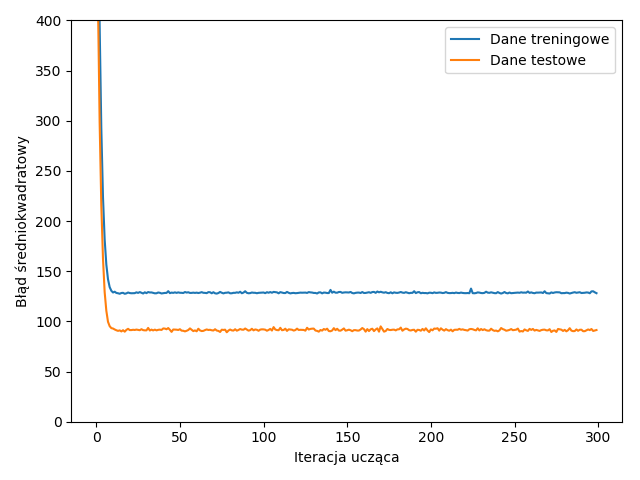
\includegraphics[width = 0.75\linewidth]{rysunki/pierwszy_model_wykres_uczenia_z_normalizacja.png}
	 		\end{tightcenter}
	 		
 			\caption{Zależność \textit{MSE} danych od iteracji uczącej dla najlepszego przypadku w pierwszym modelu ze znormalizowanymi danymi.}
			\label{fig: pierwszy_model_wykres_uczenia_z_normalizacja}
		\end{figure}
		
		\begin{figure}[h]
			\begin{tightcenter}
	 			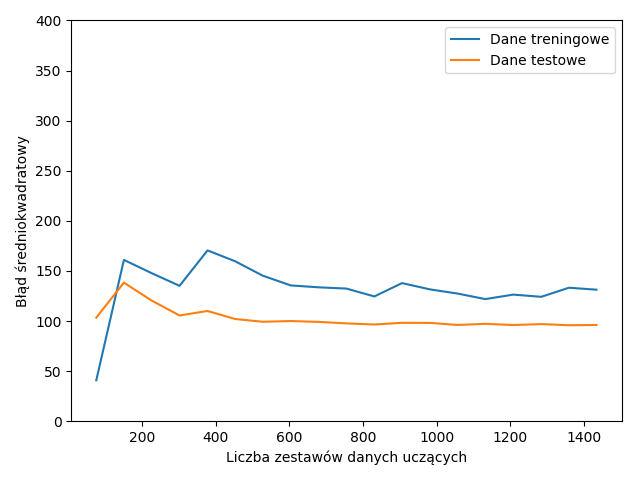
\includegraphics[width = 0.75\linewidth]{rysunki/pierwszy_model_learning_curves_z_normalizacja.png}
	 		\end{tightcenter}
	 		
 			\caption{Zależność \textit{MSE} danych od ich ilości w pierwszym modelu ze znormalizowanymi danymi.}
			\label{fig: pierwszy_model_learning_curves_z_normalizacja}
		\end{figure}
		
		Pierwszą rzeczą rzucającą się w oczy jest duża stabilność wartości na wykresach - eliminuje to sytuacje w których wynik uczenia był winą przypadku, jako że kilka iteracji wcześniej lub później \textit{Perceptron} dawał zupełnie inny rezultat. Dzięki większej stabilności sieci łatwiej jest także wyciągać wnioski na podstawie wykresów. Lepiej widoczny jest problem zauwazony wcześniej - wysoki bias modelu. Objawia się on tym, że na początku \textit{MSE} danych maleje, aż do pewnego momentu gdzie jest stały i żadna ilość danych albo długość uczenia nie spowoduje jego zmniejszenia. Ostatnią rzeczą, która jest taka sama jak w rozdziale \ref{pierwszy_model_tworzenie_i_analiza} - \textit{MSE} danych testowych jest mniejsze niż danych treningowych.
		
		\section{Drugi model - tworzenie i analiza}
		Chcąc rozwiązać główny problem mojego modelu - wysoki bias potrzebowałem modelu, który potrafi nauczyć się bardziej skomplikowanych funkcji. Takim modelem będzie sieć neuronowa z kilkoma warstwami. Dzięki każdej następnej warstwie ma ona możliwość uczenia się coraz bardziej skomplikowanych funkcji. Sieć jaką stworzyłem ma 1 warstwę ukrytą - warstwę neuronów pomiędzy wejściami a warstwą wyjść - z 30 neuronwami. Jako funkcję aktywacji wybrałem funkcję \textit{ReLU}.
		
		\printbibliography
\end{document}
